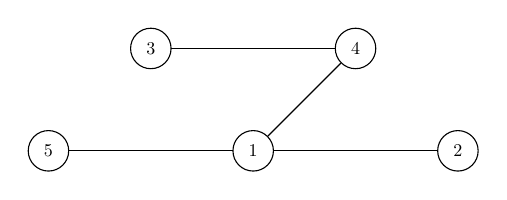
\begin{tikzpicture}[vertex/.style = {shape=circle,draw,minimum size=2.25em},scale=0.65, every node/.style={scale=0.65}]
    \node[vertex] (c1) at (0,0) {$1$};
    \node[vertex] (c2) at (4,0) {$2$};
    \node[vertex] (c3) at (-2,2) {$3$};
    \node[vertex] (c4) at (2,2) {$4$};
    \node[vertex] (c5) at (-4,0) {$5$};
    \draw (c1) -- (c2);
    \draw (c3) -- (c4);
    \draw (c1) -- (c4);
    \draw (c1) -- (c5);
\end{tikzpicture}